\documentclass[a4paper]{article}
\usepackage[utf8]{inputenc}
\usepackage[spanish, es-tabla, es-noshorthands]{babel}
\usepackage[table,xcdraw]{xcolor}
\usepackage[a4paper, footnotesep = 1cm, width=20cm, top=2.5cm, height=25cm, textwidth=18cm, textheight=25cm]{geometry}
%\geometry{showframe}

\usepackage{tikz}
\usepackage{amsmath}
\usepackage{amsfonts}
\usepackage{amssymb}
\usepackage{float}
\usepackage{graphicx}
\usepackage{caption}
\usepackage{subcaption}
\usepackage{multicol}
\usepackage{multirow}
\setlength{\doublerulesep}{\arrayrulewidth}
\usepackage{booktabs}
\usepackage{mathrsfs,amsmath}
\usepackage{hyperref}
\hypersetup{
    colorlinks=true,
    linkcolor=blue,
    filecolor=magenta,      
    urlcolor=blue,
    citecolor=blue,    
}

\newcommand{\quotes}[1]{``#1''}
\usepackage{array}
\newcolumntype{C}[1]{>{\centering\let\newline\\\arraybackslash\hspace{0pt}}m{#1}}
\usepackage[american]{circuitikz}
\usetikzlibrary{calc}
\usepackage{fancyhdr}
\usepackage{units} 

\graphicspath{./Imagenes}

\pagestyle{fancy}
\fancyhf{}
\lhead{22.05 ASSD}
\rhead{Mechoulam, Lambertucci, Rodriguez, Londero}
\rfoot{Página \thepage}

\begin{document}

\subsection{Introducción}

\subsection{Máxima frecuencia de entrada sin Sample \& Hold}

De la datasheet del ADC0808, se tiene que si $V_{CC} = V_{REF+} = 5.12V$ y $V_{REF-} = 0V$, la resolución será de $20 \frac{mV}{bit}$. Si se utiliza la frecuencia de clock $f_{CLK}$ típica utilizada en la datasheet de $640kHz$, el tiempo de conversión $t_C$ máximo será de $116\mu s$. Esto implica que la entrada no deberá de tener una pendiente mayor a $\frac{20mV}{116\mu s}$ para no introducir error en la cuantización de la señal.


Si la señal de entrada se encuentra en el peor caso, es decir, con una excursión de tensión de $-0.1V + V_{REF-}$ a $5.12V + 0.1V$; esta se encuentra montada sobre un nivel de continua igual a $(5.22V - (-0.1V))/2 = 2.66V$; y esta se puede considerar senoidal gracias a la teoría desarrollada por Fourier; se tiene que la amplitud pico máxima de la senoidal podrá ser $2.66V$. Luego, asumiendo el peor caso de la pendiente de la senoidal, para un ángulo igual a cero radianes, lo que permite utilizar la aproximación paraxial, se tiene que
\\

\begin{equation}
\left. \frac{d \left( 2.66V \cdot Sin \left( 2\pi f_{in_{max}} t \right) \right)}{dt} \right|_{t=0} = 2.66V \cdot 2\pi f_{in_{max}} = \frac{20mV}{116\mu s}
\end{equation}
\\

Finalmente, se obtiene una frecuencia máxima de $f_{in_{max}} = 10.3Hz$.
\subsection{DAC}
Se utilizó el integrad DAC0800, un conversor D/A de 8 bits con salida diferencial de corriente.
Para convertir esta corriente en un nivel de tensión se utilizó el circuito propuesto por la hoja de datos que se muestra a continuación:
\begin{figure}[H]
	\centering
	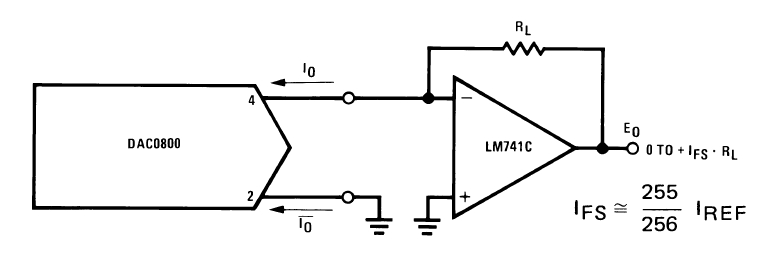
\includegraphics[width=0.8\textwidth]{ImagenesEjercicio1/dacout.png}
\caption{Configuración saldia DAC.}
	\label{fig:dacout}
\end{figure}
La salida va de 0 a $V_{fs}= I_{fs}cdot R_L$.
\end{document}